\documentclass[12pt]{article}

\usepackage{amsmath}
\usepackage{graphicx,psfrag,epsf,amssymb}
\usepackage{enumerate}
\usepackage[top=1.0in, bottom=1.0in, left=1.0in, right=1.0in, headheight=1.0in]{geometry}
\usepackage{hyperref}
\usepackage{pdfpages} % To include activity worksheets
\usepackage{float}
\usepackage{natbib}
\usepackage{enumitem}
\newlist{todolist}{itemize}{2}
\setlist[todolist]{label=$\square$}

\newcommand{\blind}{0}

\newcommand{\todo}[1]{{\color{blue}[[\textbf{TODO: }#1]]}}

\date{December 15, 2019}

\begin{document}
\def\spacingset#1{\renewcommand{\baselinestretch}%
{#1}\small\normalsize} \spacingset{1}


%%%%%%%%%%%% DEFINING TITLE FOR PAPER & REMOVAL FOR BLIND VERSION %%%%%%%%%%%%%%

\if1\blind
{
  \title{\bf Designing Data Science Workshops for Data-Intensive Environmental 
  Science Research}
  \author{Allison Theobold \thanks{The authors gratefully acknowledge the 
  \textit{National Network of Library of Medicine}
    Data Engagement PNR grant for supporting this research.} \hspace{.2cm}\\
    Department of Mathematical Sciences, Montana State University \\
    Bozeman, MT \\
    allisontheobold@montana.edu \\
    and \\
    Stacey Hancock \\
    Department of Mathematical Sciences, Montana State University \\
    stacey.hancock@montana.edu \\
    and \\
    Sara Mannheimer \\
    Montana State University Library \\
    sara.mannheimer@montana.edu
    }
  \maketitle 
} \fi

\if0\blind
{
  \title{\bf Designing Data Science Workshops for Data-Intensive Environmental Science Research}
  \author{Anonymous}
  \date{}
  \maketitle
} \fi
%%%%%%%%%%%%%%%%%%%%%%%%%%%%%%%%%

\bigskip

\begin{abstract}
% currently 186 words 

Over the last 20 years, statistics preparation has become vital for a broad 
range of scientific fields, and statistics coursework has been readily 
incorporated into undergraduate and graduate programs. However, a gap remains 
between the computational skills taught in statistics courses and those required
for the use of statistics in scientific research. Ten years after the 
publication of ``Computing in the Statistics Curriculum,'' the nature of 
statistics continues to change, and computing skills are more necessary than 
ever for modern scientific researchers. In this paper, we describe research on 
the design and implementation of a suite of data science workshops for 
environmental science graduate students, providing students with the skills 
necessary to retrieve, view, wrangle, visualize, and analyze their data using 
reproducible tools. These workshops fill a critical hole in the environmental 
science and statistics curricula, supporting students with opportunities to grow
in their skills for computing with data. Open to faculty, staff, and the larger
community, these workshops promote continued learning of the tools necessary for
working with data and provide additional resources for incorporating data 
science into the classroom.

\end{abstract}

\noindent %
{\it Keywords:}  data science, data visualization, data wrangling, \texttt{R}, 
environmental science, workshops, reproducible research 

\vfill

\newpage
\spacingset{1.45}

\section{Introduction}
\label{sec:intro}

\quad Scientific fields have seen profound increases in the volume and variety 
of data available for analysis. Matched with the growth in computational power, 
today's scientific researchers are faced with computational and statistical 
expectations beyond those of the coursework dictated by their curriculum. In the
environmental sciences, though statistics courses have been readily incorporated
into undergraduate and graduate curricula, an abundance of literature suggests 
that these curricula fail to equip graduate students with the computing skills 
necessary for research in their field (Andelman et al., \citeyear{andelman}; 
Green et al., \citeyear{green}; Hampton et al., \citeyear{hampton}; Hernandez et
al., \citeyear{hernandez}, Mislan, Heer, \& White, \citeyear{mislan}; Teal et 
al., \citeyear{datacarpentry}; Theobold and Hancock, \citeyear{theobold}). Only 
one of these studies \citep{theobold}, however, acknowledges the substantial 
role statistics courses could potentially play in students' acquisition of 
computational skills. 

\quad Over the last 10 years, a large number of statistics educators have echoed
Nolan and Temple Lang's call to ``embrace computing and integrate it fully into 
statistics undergraduate major and graduate programs" (Nolan and Temple Lang, 
\citeyear{nolan}, p. 97; Baumer, \citeyear{baumer_datascience}; Baumer, Horton, 
\& Wickham, \citeyear{horton_takingachance}; Cetinkaya-Rundel and Rundel, 
\citeyear{mine}; Cobb, \citeyear{cobb}; Hardin et al., \citeyear{hardin}; Horton
and Hardin, \citeyear{horton_thinkwithdata}; Kaplan, \citeyear{kaplan}; McNamara
and Horton, \citeyear{mcnamara}). Indeed, the American Statistical Association 
Curriculum Guidelines for Undergraduate Programs in Statistical Science 
\citep{asa} reflect the increasing importance of data science skills. Despite 
this campaign for computing in the statistics classroom, graduate-level 
statistics service courses have largely been overlooked, even though their 
potential impact is substantial. Unlike courses designed for an undergraduate or
graduate program in Statistics, these service courses often act as the sole 
exposure to computing with data prior to the start of a student's independent 
research. 

\quad The intention of this research is to (1) describe the computing skills 
necessary for research in the environmental sciences, (2) investigate how these 
skills can be infused into currently existing extracurricular workshops, and (3)
understand the experiences of attendees of these workshops. We consider the 
following research questions:
\begin{enumerate}
    \item What do environmental science faculty members identify as the key 
    computing skills graduate students require to implement statistics for 
    research in their field?   
    \item How can the key computing skills identified by environmental science 
    faculty be incorporated into currently existing workshop materials?  
    \item What are the experiences of individuals attending data science 
    workshops?  
\end{enumerate}

\quad To investigate these questions, we executed a three-phase design-based 
implementation research model \citep{penuel}. In the first phase, we conducted 
in-depth interviews with faculty from environmental science fields regarding the
computational skills they believe are necessary for graduate students to succeed
in their research. Phase two then focused on adapting currently existing 
workshop resources to design of a series of data science workshops targeting the
key computational skills distilled from these interviews. The final phase 
consisted of implementing the workshops and collecting survey responses from the
workshop attendees regarding their experiences participating in each workshop.  

\begin{figure}[h!]
    \centering
    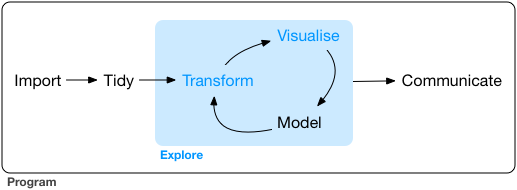
\includegraphics[width = \textwidth, height = 2in]{images/data-science-explore.png}
    \caption{Data Analysis Cycle, Wickham, H. \& Grolemund, G. (2017) \emph{R 
    for Data Science}. Sebastopol, California: O'Reilly.}
\label{fig:cycle}
\end{figure}

\quad For this research, the collection of disciplines who perform research 
across a variety of environmental science fields are captured under the term 
``environmental science.'' At our institution, these are the fields of Ecology, 
Land Resources Environmental Sciences, Plant Sciences, and Animal and Range 
Sciences, whose students are required or highly recommended to complete 
graduate-level statistics coursework for a masters or doctoral degree. In this 
paper, the ``data analysis cycle'' consists of all stages in the data analysis 
process, from data importation to data exploration to the communication of 
results, where data modeling is but one component (Figure \ref{fig:cycle}). 
The ``data science skills'' necessary to engage in this cycle may include 
general programming concepts such as loops, user-defined functions, or 
conditional statements. However, the cornerstone of data science skills differs
fundamentally from general programming skills, with a focus on data rather than 
computer architecture, design, and applications. 

\quad We begin by outlining areas of research that address the computational and
statistical training of graduate students in the environmental sciences and the 
potential for extracurricular workshops to fill in the gaps. Next, we outline 
the design-based implementation research methodology used to design and 
implement a suite of data science workshops tailored to environmental science 
graduate students. Section \ref{sec:design} summarizes the first phase of 
research, which outlined the computational skills faculty members identified as 
necessary for graduate students to succeed in their independent research. Next, 
Section \ref{secion:workshops} discusses how these identified skills were 
interwoven into existing data science workshop materials for researchers in the 
environmental sciences. Section \ref{sec:implement} summarizes the backgrounds 
and experiences of the workshop attendees during the 2018-2019 academic year, 
and describes the research conducted on the implementation of the workshops. We 
then outline future research plans for a second iteration of this design work. 
To close, we revisit the current climate of computing in the statistics 
curriculum for service courses and describe how these types of extracurricular 
workshops can assist in further integration of computing into these classrooms. 

\section{The Current Climate of Statistics and Computing in the Environmental 
Sciences}
\label{sec:lit}

\quad Due to the substantial growth in the volume and variety of available data 
over the last two decades, the practice of environmental science has changed 
dramatically. Advances in technology have made computationally heavy 
applications of data science techniques---such as management and coalition of 
large data sets, high frequency spatial and temporal data visualization, and 
hierarchical Bayesian modeling---essential understandings for environmental 
science research. This flood of data has ``challenged the research community's 
capacity to readily learn and implement the concepts, techniques, and tools" 
\citep[p. 546]{hampton} necessary for data-intensive environmental science 
research, creating a crucial need to re-evaluate how our educational system can
better prepare current and future generations of researchers 
(\citeauthor{green}, \citeyear{green}; \citeauthor{hampton}, 
\citeyear{hampton}).  

\subsection{Computing in the Environmental Sciences Curriculum}

\quad Arising from a decade of mumblings \citep{andelman, dodds1, dodds2, eglen, 
green, hastings, kelling, wilson-software-carpentry, wilson, wing}, 2010 brought
two studies on the computational ill-preparation of environmental students by
their curriculum. First, Strasser and Hampton found that undergraduate students
were not being prepared with the data management tools necessary to engage in
environmental science research, as fewer than 20\% of instructors were including
key data management topics in their courses, such as workflows, databases,
and reproducibility. The importance of these skills, however, was affirmed by
the majority (77\%) of instructors. Yet, instructors largely stated that ``data
management should be taught in a different course'' (p.\ 10). The results of 
this study suggested that---across institutions---``data management education
is not currently a priority for ecology instructors'' (p.\ 10). That same year,
an environmental science graduate student led a large scale study of the
computational experiences of future environmental scientists 
\citep[p.\ 1068]{hernandez}. In a survey of environmental science graduate 
students across the United States, the authors found that over 74\% of the
students surveyed reported they had no skills in any programming 
language---including \texttt{R}---and only 17\% reported basic skill levels in
any programming language. Hence, a large number of students may be leaving their
graduate programs without the data science skills necessary for data-intensive
research in their field. Hernandez et al.\ suggested that student-focused
workshops could bridge this gap, by ``providing intensive environments'' where
students could learn ``particular methods or technologies'' (p.\ 1075). The
authors also noted that developing and offering these workshops would be simpler
than developing new courses to organize and implement. 

\quad Out of these calls for high-quality resources for scientific computing, 
emerged the Carpentries project \citep{carpentries}. Housing Data, Software, and
Library Carpentry, the Carpentries comprises ``communities of instructors, 
trainers, maintainers, helpers, and supporters'' all sharing the mission to 
``teach foundational computational and data science skills to researchers.'' 
These workshops address the need for ``good training resources for researchers 
looking to develop skills that will enable them to be more effective and 
productive'' \citep[p.\ 135]{carpentries}. Furthermore, these workshops are 
necessary, because ``training in data and computing skills is still largely 
absent from undergraduate and graduate programs,'' so ``most or all of what 
[researchers] know about data management, analysis, and sharing has been learned
piecemeal, or not learned at all'' (p.\ 136). Data Carpentry provides 
domain-specific training for researchers in the ``core data skills for 
efficient, shareable, and reproducible research practices'' 
\citep{data-carpentry}.  As part of this mission, the Carpentries
collaboratively develops publicly available lessons for specific populations
of researchers, which do not assume that attendees have any prior knowledge
before attending the workshops. Teal and colleagues acknowledge that, while 
the Data Carpentry workshops ``will not be able to teach researchers all of the
skills they need in two days,'' the workshops ``are a way to get started,''  
lowering the activation energy required and empowering researchers ``to be able
to conduct the analyses necessary for their work in an effective and 
reproducible way'' (p.\ 143). The success of these workshops can be viewed as 
a ``symptom of the current curriculum's shortcomings'' \citep[p.\ 547]{hampton}, 
as there continues to exist a ``paucity of systematic training within university
programs to equip students with the computational skills they need to conduct 
data-intensive research'' (p.\ 547). 

\quad Disappointingly, none of these conversations have acknowledged the 
substantial role students' statistics education potentially plays in their 
attainment of the data science skills necessary for research. Hampton and 
fellow environmental science researchers claim that ``three decades ago, 
environmental scientists were ill-prepared to use statistics in their research, 
and now statistics preparation is considered vital." In fact, in ecology today,
it is ``extremely difficult to publish a manuscript without any statistical 
testing'' \citep[p. 547]{hampton}. Furthermore, with the invention 
of the RStudio integrated development environment \citep{rstudio}, the software 
used throughout the data analysis cycle by environmental science researchers has
changed. In 2017, the number of studies in environmental science journals 
reporting the use of \texttt{R} as the ``primary tool reported in data 
analysis'' was 58\%, compared to 11.4\% in 2008 \citep[p. 1]{Rpopular}. 
Moreover, the preponderance of environmental science graduate students are now 
required to produce code as part of their research \citep{mislan}. The clear 
need for data science proficiency in environmental science research requires a
transformation of the graduate curriculum similar to that which infused
statistics preparation into the required graduate coursework. 

\subsection{Computing in the Statistics Curriculum}

\quad Changes in the digital age have also had ``a profound impact on statistics
and the nature of data analysis" \citep[p. 97]{nolan}, with today's skills 
differing substantially from what was needed but five to ten years ago. 
In the year following the publication of ``Computing in the Statistics 
Curriculum'' \citep{nolan}, the Mckinsey Report \citep{mckinsey} was published. 
The McKinsey report stated that, by 2018, ``the United States alone could face a
shortage of 140,000 to 190,000 people with deep analytical skills as well as 1.5
million managers and analysts with the know-how to use the analysis of big data
to make effective decisions'' (p.\ 3). With calls to transform the undergraduate
statistics curriculum resounding nationally, the 2014 American Statistical 
Association (ASA) President, Nathaniel Schenker, convened a workgroup to update
the association's guidelines for undergraduate programs. These new guidelines 
included an increased emphasis on data science skills and real applications, 
specifically students' ability to ``access and manipulate data in various ways,
use a variety of computational approaches to extract meaning from data, program
in higher-level languages" \citep[p.\ 7]{asa}. 

\quad With this curricular momentum, in 2015, \emph{The American Statistician} 
produced a special issue on ``Statistics and the Undergraduate Curriculum,'' to
encourage submissions of broader topics in the statistics curriculum. Articles 
in the special issue ranged from detailing how computing should be included 
throughout the Statistics curriculum \citep{jenny, tintle, hesterberg}, to 
presenting thoughts on how data science topics should be integrated into 
undergraduate statistics courses, \citep{nolan-data-analysis, grimshaw, 
baumer_datascience, hardin}. In the same issue, George Cobb provocatively stated
that the statistics curriculum needed to be rebuilt ``from the ground up'' 
(\citeyear{cobb}), as ``what we teach lags decades behind what we practice'' and
``the gap between our half-century-old curriculum and our contemporary 
statistical practice continues to widen'' (p.\ 268). Moreover, despite the 
issue's focus on the broader statistics curriculum, authors continued to lament 
that the current Introductory Statistics curriculum teaches a snapshot of the 
entire data analysis cycle, ``wherein challenges with data computational 
methods, and visualization and presentation are typically elided'' 
\citep[p.\ 336]{baumer_datascience}. 

\quad The following year, however, brought the revised GAISE college report 
\citep{gaise}, creating a push for reform in the Introductory Statistics 
curriculum. The six recommendations originally outlined by the committee in 2005
continued, but the authors suggested two new emphases for the first
recommendation (teach statistical thinking), which reflect the modern practice
of statistics. First, statistics educators should ``teach statistics as an
investigative process of problem-solving and decision making,'' and we should 
``give students experience with multivariable thinking'' (\citeyear{gaise}, 
p.\ 3). These recommendations reiterate the sentiments heard throughout the
statistics community, that students should emerge from our courses with the
understanding that data analysis ``isn't just inference and modeling, it's also
data importing, cleaning, preparation, exploration, and visualization'' 
\citep{mine-jsm}. Yet, the inclusion of these topics in the Introductory 
Statistics curriculum is still a heated discussion. Many educators continue to 
believe (1) that it is not possible to teach statistical concepts and 
programming in just one course, (2) that teaching programming takes up valuable
time which could be used towards teaching important statistical concepts, or 
(3) students are not interested in learning to program \citep{mine-jsm}. Thus, 
many students leave their Introductory Statistics course without ``a set of 
practices and attitudes about data that are immediately applicable to their 
lives'' \citep[p.\ 309]{gould}. 

\quad Amidst these conversations, \texttt{R} packages were being created, which 
would fundamentally changing how users interact with \texttt{R}. These 
\texttt{R} packages, universally known as the ``\texttt{tidyverse},'' have 
created user friendly \texttt{R} tools which ``share an underlying design 
philosophy, grammar, and data structures'' \citep{tidyverse}. Statistics 
educators have begun to leverage these tools in the Introductory Statistics 
classroom to teach reproducibility \citep{mine-rmarkdown}, data management 
\citep{horton_takingachance}, dynamic data \citep{hardin-tise}, and big data
\citep{horton-tise}. While there exists a growing momentum to incorporate these
new \texttt{R} tools into the Introductory Statistics classroom, attention has 
yet to be paid to alternative statistics service courses, such as those taken 
by environmental science graduate students. These courses, like Introductory 
Statistics, serve graduate students from a variety of scientific backgrounds. 
However, unlike an undergraduate Introductory Statistics course, students are 
expected to emerge from their statistics coursework with the ability to 
complete the analyses required for their research. 

\quad The frustrations echoed by environmental science educators 
\citep{hampton, datacarpentry} suggest that, despite the inclusion of statistics 
coursework into these graduate programs, students continue to leave the 
statistics classroom without the data science skills necessary to participate in 
the data analysis cycle in their own research. The fundamental question raised 
ten years ago by Nolan and Temple Lang still applies today: do our students
leave the statistics classroom able to ``compute confidently, reliably, and
efficiently?'' (\citeyear{nolan}, p.\ 100). An in-depth study of environmental 
science graduate students' experiences acquiring the computing knowledge
necessary for their research answered this question with a resounding `no' 
\citep{theobold}. Like the hypothesis of Teal and colleagues (2015), these
students did not attribute their acquisition of the data science skills
necessary for their research to the statistics courses they took for their
degree. Rather, students gained the data science skills necessary to engage in
the entire data analysis cycle through independent research experiences, an
``all-knowing'' past or current graduate students, and peer networks. Ten years 
after the publication of ``Computing in the Statistics Curriculum,'' we continue
to assume that ``students will `pick up' the skills they need'' to participate 
in the data analysis cycle outside of their statistics coursework 
\citep[p.\ 309]{gould}. 


\subsection{Extracurricular Workshops to Bridge the Gap}

\quad Reiterated by both statistics education and environmental science 
researchers alike \citep{nolan, datacarpentry}, this lack of training in 
computational skills impedes the progress of scientific research, sends the 
signal to students that computing is not of intellectual importance, and is 
laden with hidden costs. Students may pick up bad habits, misunderstandings, or 
the wrong concepts, learn just enough to get what they need done, spend weeks or
months on tasks that could be done in hours or days, and they may be unaware of 
the reliability and reproducibility---or lack there of---of their results (Nolan
and Temple Lang, 2010, p. 100; Teal et al., 2015, p. 136). But why are these
skills still so rarely included in these service courses when the need for them
is widely recognized?

\quad Environmental science educators have reiterated the challenges in 
integrating computing into the curriculum outlined by Nolan and Temple Lang. 
These barriers can be boiled down to ``attempting to fit more material into
already-full courses and curriculum, which are taught by people who do not feel
prepared to address topics relevant to big data and data-intensive research'' 
\citep[p. 547]{hampton}. These hurdles are potentially even greater for 
graduate-level statistics service courses. Instructors of these courses are 
explicitly told the statistical content students are expected to learn, 
and are implicitly assumed to be teaching students the data science skills 
necessary for them to participate in the entire data analysis cycle. Claiming 
these graduate students ought to take additional, data science specific courses
to obtain these skills is infeasible for many, as graduate programs leave little
room for additional coursework. 

\quad Until computing has been meaningfully integrated into these service 
courses, extracurricular workshops hold the potential to address the gap between
the computational preparation of students by their coursework and the 
computational requirements of their research. Extracurricular workshops are
not a direct substitute for the prolonged instruction of these skills that
occurs in a course. But, short, intensive workshops, such as those provided by 
the Carpentries, are able to teach immediately useful skills that can be taught
and learned quickly, keep learners active by using live coding and formative 
assessment, work with a learners from a variety of backgrounds, and build
learners' self efficacy \citep{null-carpentries}. Additionally, because
workshops are able to thrive outside of university curricula, they hold the
ability to ``adapt materials rapidly and remain on the leading edge of
technological development'' \citep[p. 547]{hampton}. Furthermore, workshops
offer the opportunity for a wide variety of researchers, not just students, to
acquire the data science skills necessary for data-intensive research, 
supporting the broader community of researchers. 

% \quad Improving environmental science graduate students' access to ``powerful, 
% effective learning opportunities'' \citep[p. 137]{penuel} necessitates 
% understanding the skills required for these students to be successful in their 
% research. As the direct supervisors of graduate students, environmental science 
% faculty members are aware of the computing skills that are vital to researchers
% in their respective fields. Through interviews with these faculty members, we
% gain an understanding of the essential skills required of environmental science
% graduate students, which allows us to tailor the Carpentries content to meet the
% needs of this community. Furthermore, the process of iterating through multiple
% offerings provides the opportunity to incorporate feedback and to revise the
% lessons, yielding high-quality training to graduate student researchers in these
% fields. 

\section{Design-Based Implementation Research} 

\quad Design-based implementation research (DBIR) ``offers a model for the 
design and testing of innovations within the crucible of classrooms and other 
contexts for learning'' (Cobb et al., \citeyear{confrey}; Fishman et al., 2013, 
p. 140; O'Neill, \citeyear{oneill}). This model of research emphasizes the 
iterative process of design and evaluation and is particularly well suited for 
research that develops ``evidence-based improvements to innovations,'' where 
evidence from the implementation informs changes made to these innovations for 
learning. Similar to other forms of design research, DBIR ``uses research to 
solve practical problems'' \citep[p. 143]{penuel}, but focuses on the 
development and evaluation of ``usable tools for improving teaching and learning
in specific subject matter domains and settings'' (\citeauthor{confrey}, 2003;
Fisherman et al., p. 143). Additionally, the collaborative nature of design 
research positions members of the community as ``co-designers of solutions to 
problems'' \citep[p. 140]{penuel} rather than bystanders. 

% Because the aim of this research was to develop and offer data science workshops for a specific community of researchers, a large number of faculty in these fields have contributed to this research and are aware of the workshops, encouraging students in their courses to attend. When creating workshops for a broader community of researchers, we encourage Statisticians to build connections with faculty in these fields, to better understand the needs of their students. The discipline of Statistics was developed to support research in other scientific disciplines to evaluate evidence obtained from data, a position we should heed when developing resources for researchers in the broader scientific community.

\quad The first iteration of this DBIR consisted of three phases. The first 
phase focused on investigating the computing skills necessary for environmental 
science research by graduate students. For phase two, the skills identified 
during phase one were used to design data science workshops for graduate 
students in the environmental sciences, using currently existing Data and 
Software Carpentry lessons \citep{carpentries}. The final phase focused on
evaluating the developed data science workshops, after their first
implementation. In this first iteration of our DBIR, the data collected from the
workshop attendees' focus on their backgrounds prior to the workshop, previous
experiences learning \texttt{R}, and their experiences in the workshop, rather
than the learning outcomes of the workshop attendees. 

\quad The phases of this research, the research question each phase addresses, 
and the data collected during each phase are outlined in Table \ref{tab:phases}. 

{\spacingset{1.05}
\begin{table}[h!]
\centering
\begin{tabular}{p{10cm}p{2cm}p{3cm}}
\hline
Research Question & Design Phase & Data Collected  \\
\hline
What do environmental science faculty members identify as the key computing skills graduate student require to implement statistics in environmental science research?   &  Phase 1 & Faculty interviews \\ \vspace{0.1cm}

How can the key computing skills identified by environmental science faculty be incorporated into currently existing workshop materials?  & Phase 2 & Carpentries curriculum materials  \\ \vspace{0.1cm}

What are the experiences of individuals attending data science workshops?  & Phase 3 & Pre- and post-workshop surveys \\
\hline
\end{tabular}
\caption{Research questions, phases, and data collected for the three-phase DBIR.}
\label{tab:phases}
\end{table}
}

\section{Computing Skills Necessary for Environmental Science Research}
\label{sec:design}

\quad Phase one of this research investigated the computational skills necessary
for graduate students in the environmental sciences to implement statistics in
their research. These needs were explored through interviews with faculty
members who directly supervise graduate student researchers in the environmental
sciences. 

\subsection{Participants}

\quad In the spring of 2017 and fall of 2018, faculty members from diverse 
fields within the environmental sciences were invited to participate in a 
one-hour interview. All faculty members currently overseeing a graduate student
from the Ecology, Land Resources Environmental Science, Animal \& Range 
Sciences, and Plant Sciences \& Plant Pathology departments were emailed 
requesting their participation in this research. While some faculty 
enthusiastically agreed to participate, others declined for three main 
reasons---they hadn't directly overseen a graduate student recently, they deemed
themselves to be weak in statistics, or they were unavailable to meet. Table 
\ref{tab:faculty} outlines the number of faculty requested for participation and
the number of faculty interviewed, by department affiliation. 

{\spacingset{1.05}
\begin{table}[h!]
\centering
\begin{tabular}{lcc}
\hline
Department & Faculty Invited & Faculty Interviewed  \\
\hline
Animal \& Range Sciences & 7 & 2 \\
Ecology & 15 & 8 \\
Land Resources Environmental Sciences & 24 & 8 \\
Plant Sciences \& Plant Pathology &  15 & 5 \\ 
\hline
\end{tabular}
\caption{Number of faculty members requested for participation and interviewed,
by department.}
\label{tab:faculty}
\end{table}
}

\subsection{Data Collection}  

\quad Faculty agreeing to participate were interviewed regarding (1) the 
computational skills they believe are necessary for masters and doctoral 
students to implement statistics for research in their field, and (2) how they 
believe graduate students acquire these necessary skills. The full interview 
protocol is included in Appendix A.  

\quad Based on faculty's responses, the interviewer asked follow-up questions to
further explore why the faculty believe the computational skill(s) in question 
are necessary. For instance, if a faculty voiced the need for students to be 
able to build a data workflow, further information was sought regarding what 
specific computing skills this would require. Alternatively, when the response 
from faculty consisted of the statistical understandings necessary for graduate
student researchers, follow-up questions were asked to delve further into what
computing skills a student may require to successfully implement this type of
statistical analysis with their data. Not only did these interviews provide
valuable feedback on \emph{what} content the workshops should include, they also
added insight into \emph{why} workshops form the ideal mode of delivery for this
needed training.  

\subsection{Data Analysis} 

\quad The primary author lead a three-stage data analysis process (Miles, 
Huberman, Salada$\tilde{\text{n}}$a, \citeyear{miles}). During the first stage,
the interviews for every faculty member were transcribed verbatim. Following 
this process, the primary author read the transcripts independently, 
highlighting excerpts where computing skills were discussed. The author then 
created descriptive codes for the skills faculty identified as necessary in each
of these excerpts. At the close of this stage, the author examined these codes 
for specific references to computing skills currently addressed in Data 
Carpentry's \emph{Data Analysis and Visualization in \texttt{R} for Ecologists} 
lesson. This lesson ``uses a tabular ecology dataset from the Portal Project 
Teaching Database and teaches data cleaning, management, analysis, and 
visualization" \citep{ecology_curriculum}. 

\quad Following this process, the primary author began the second stage of 
analytical coding. This stage acts as a method of synthesizing descriptive 
summaries, tying together ``different pieces of data into a recognizable 
cluster,'' demonstrating how the data are instances of a general concept 
\citep[p. 95]{miles}. During this stage, skills were linked thematically, and 
categories that held across multiple interviews were retained. For example, 
every faculty voiced students' need to work with data in \texttt{R}. These 
themes were initially categorized as ``working with data,'' with additional 
categories of data wrangling, and data visualization created. Next, the author
searched through these themes to uncover how each theme related to the others.
Through this process it was determined that certain categories captured similar
constructs, and were merged into a single category, whereas other constructs
were voiced independently, and separate categories were formed. For example,
while every faculty voiced students' need to work with data in \texttt{R}, these
sentiments were voiced alongside students' need to preform other data wrangling
operations, such as reorganize data, filtering out rows of data, selecting
columns, creating new variables, or modifying existing variables. Hence, the
themes of ``working with data'' and ``data wrangling'' were merged into the
single theme of ``working with data.'' Alternatively, while reproducibility is
a key aspect to working with data in \texttt{R}, the skills identified by
faculty which this theme captures were not voiced alongside a specific software.
However, when these faculty commented on the need for students' work to be 
reproducible, \texttt{R} was continually mentioned as the vehicle to support 
this need. 

\quad In the final stage of the analysis, the primary author searched the 
faculty transcripts for evidence supporting the emerging themes, scrutinizing 
whether each identified skill fit into the existing themes. Following this 
validation process, the first and second authors met to discuss the rationale
for each code and inspect the skills identified by faculty in the context of the
emergent themes. These final themes ground the theory for creating an effective
intervention promoting the acquisition of computing skills necessary for 
graduate-level environmental science research. reproducible
research

\subsection{Skills Identified by Environmental Science Faculty}

\quad While some faculty had difficulties disentangling the statistical methods
students use in research from the computing required to implement those methods,
many were able to express the expectations they held for graduate students in
their field throughout the entire data analysis cycle. These faculty member
expectations fell predominantly into three categories: (1) working with and
wrangling data, (2) data visualization, and (3) reproducibilty.

\subsubsection{Working with Data}  

\quad All of the faculty interviewed believed that students' experiences in the
statistics classroom do not adequately prepare students to work with and
organize large, messy datasets. The need to manipulate large datasets is not
unique to the environmental sciences. In fact, a faculty member stated that it
is ``not uncommon to be analyzing half a million records, but I think it's
uncommon to be doing it effectively or efficiently.'' As graduate students
perform their research, they are required to assemble datasets for analyses.
This requires students to think about ``storing data, managing data, matching
data, and collating data," potentially merging a variety of data types into one
meaningful data set. Every faculty member emphasized that students need to know
how to ``organize their data and get it in a way that can be used by 
\texttt{R}.'' 
  
\quad Often included in these skills for working with data are tasks that 
require reorganizing data formats from wide to long or vice versa---a skill 
which every faculty member griped is not acquired through the standard 
curriculum. ``Most of them, when you're like `long form, wide form, samples as 
rows, variables as columns,' they kind of look at you like `what?'.'' Standard 
examples in statistics courses provide students with data which are the product
of cross-tabulation, so students are never forced ``to figure out how to get the
cross-tabulation you need, so that you can bring it into \texttt{R} and do your
regression.''

\subsubsection{Data Visualization} 

\quad The importance data visualization plays in every stage of students'
research was emphasized by every faculty member interviewed. Faculty affirmed
that students should possess the ability to create visualizations of their data
early, both for checks of data quality and to explore relationships. One faculty
member declared that students' ability to look at their data in different ways
dramatically shapes their research potential, and the tools available today 
allow for researchers to create visualizations precisely tailored for each
investigation. Many faculty voiced the usefulness of the \texttt{ggplot2} 
\citep{ggplot} package for students' knowledge of producing data visualizations,
lowering the barrier for students to learn ``how to visualize [their] data to
explore and understand it.'' 

\subsubsection{Reproducibility}  

\quad Every faculty member emphasized the usefulness of ``manipulating data in
ways that are repeatable,'' through using such programs as \texttt{R}. Across
environmental science disciplines, faculty concurred that many students do not
use \texttt{R} for data wrangling. Instead, students rely on Excel because 
``they are not comfortable enough with the code or [\texttt{R}] is kind of a 
black box'' or that when they ``don't have that instant connection with [their]
data, I think it fundamentally boils down to fear.'' Concern was raised for the
students using Excel to wrangle their data, as ``they would never find [their]
way back to what the original data set would have been'' and that their advisers
would have no way to understand why data are missing. These advisers encourage
students to avoid these brute force Excel manipulations, but students may not
have the computing skills necessary to perform the same data wrangling task in a
scripted and reproducible manner in \texttt{R}.

\subsubsection{How Students Gain Computational Skills}

\quad When asked why students are not acquiring computing skills in the courses
required for their degree, a faculty member stated, ``We don't really have
anyone to teach that. It's not that it isn't valuable, but there is no one to
teach it.'' When pressed as to why other faculty feel uncomfortable teaching
computing, this same faculty member stated, ``[they believe] most graduate
students come in knowing more about the tools one might use to manipulate data
than their advisers do.'' Other faculty bemoaned the gaps between the
computational skills of their graduate students and their own training, 
``I think that more and more in our field, my generation is sort of just 
catching up the next generation.'' These gaps impact the assistance faculty can
provide to their students, as ``increasingly faculty feel that they're not at 
the forefront of their programming abilities, so their students are being 
self-taught and are often computationally ahead of them.'' Many faculty 
lamented their own deficient computational abilities, with some stating that 
they ``feel personally out of touch, because [students] work in \texttt{R} and 
I haven't taken the time to learn \texttt{R}, because of my training and my
age.'' These faculty understand that often students are required to learn these
skills on their own because ``there is definitely a gap between the code I can
help them with.''  

\quad Although faculty feel that there may exist gaps between their own
knowledge of working in \texttt{R} and their students', every faculty member
affirmed the importance of students acquiring the computational abilities needed
to perform data-intensive research. Indeed, it is not necessary for every
student to be an expert, but faculty underscored the value of resources for
students to acquire these computational skills necessary for their research. The
majority of faculty voiced that it is often assumed that graduate students
should be able to analyze their data because they've taken a statistics course.
Yet, faculty members acknowledge the poor computational preparation of their
students even after taking a statistic course, and thus ``encourage [students]
to use anything they can find to get more tools in [their] tool box.'' 

\section{Designing Data Science Workshops for Graduate Students in the 
Environmental Sciences}
\label{secion:workshops}

\quad The second phase of this research attended to the  development of a suite of data science workshops targeted to graduate students in the environmental sciences. Skills identified through faculty interviews were incorporated into a set of four 3-hour workshops covering (1) the basics of programming in \texttt{R}, (2) intermediate programming tasks in \texttt{R}, (3) creating appropriate and effective data visualizations, and (4) cleaning and merging data in preparation for analysis and visualization, all using reproducible tools. 

\quad The first workshop does not assume that attendees have any previous experience working in \texttt{R}, and each workshop builds on the knowledge acquired at previous workshop(s), without the expectation that attendees have acquired additional knowledge or skills between workshops. The materials from these workshops were adapted from Data Carpentry's \emph{Data Analysis and Visualization in \texttt{R} for Ecologists} lesson \citep{ecology_curriculum} \footnote{This work is a derivative of Data Analysis and Visualization in \texttt{R} for Ecologists \href{https://datacarpentry.org/R-ecology-lesson/}{(https://datacarpentry.org/R-ecology-lesson/)} by Data Carpentry, used under CC BY \href{https://creativecommons.org/licenses/by/4.0/}{(https://creativecommons.org/licenses/by/4.0/)}.}, incorporating additional skills environmental science faculty identified as necessary for graduate students to succeed in their research.   

% This work is a derivative of Elephant@Amboseli (https://datacarpentry.org/R-ecology-lesson/) by Data Carpentry, used under CC BY (https://creativecommons.org/licenses/by/4.0/).

\quad Data Carpentry is a component of the Carpentries project, with curricula developed to support research in ecology, genomics, and the social sciences. Data Carpentry workshops create an excellent starting point for designing a workshop curriculum for environmental science graduate students, as the Ecology curriculum is maintained by experienced researchers in that field, using field-specific data contexts. Using the themes which emerged in interviews with environmental science faculty, we were able to tailor \emph{Data Analysis and Visualization in \texttt{R} for Ecologists} to best suit the needs of this population of graduate students as they prepare for and participate in data-intensive research. The workshop materials developed for this research are publicly available through GitHub, 
%\footnote{\href{https://github.com/atheobold/data-science-workshops-jse}{GitHub repository (link)}}
with video tutorials recorded and available through our institution's library.   %\footnote{\href{http://www.montana.edu/datascience/training/index.html#workshop-recordings}{MSU Library Videos (link)}}.  

\subsection{Participant-Centered Learning}  

\quad These workshops are taught in a technology-enhanced active learning (TEAL) classroom that seats up to 35 individuals. The classroom has two monitors on every wall, a projector at the front of the room, and tables that seat groups of three to four persons. The layout of the room allows for every student to watch as the instructor live codes, and supports the instructor and workshop assistants to easily engage with attendees as they work. Each workshop has one lead instructor and two to three workshop assistants. The assistants are tasked with addressing any participant questions that may arise during the workshop.  

\quad During the workshop, every topic is first introduced by the instructor, followed by the live coding of an example. The group then engages in a discussion of the method. This group dialogue creates an inclusive space where attendees are able to pose questions or conjectures to the group while the instructor live codes questions asked or suggestions. Finally, attendees group up to complete a set of hands-on tasks, applying the concepts covered in that section of the workshop. These tasks allow for attendees to ``learn the computational aspects as part of an interesting, challenging, and confidence-building process'' \citep[p. 101]{nolan}. As attendees work in groups to tackle the task at hand, they are instructed to place a colored sticky note on their computer, to signal assistants for help.    

\subsection{Data Context}  
\quad Faculty emphasized the importance of students acquiring computing skills in familiar data contexts. Therefore, the data used in the creation of these workshops are ecological data sets, originating from Montana Fish, Wildlife, and Parks and the Portal Project Teaching Database \citep{portal_data}. These data highlight a variety of aspects that commonly occur in environmental data, including multiple sampling instances, mark-recapture, biological measurements, and meta- and micro-level data. 

\quad The data from Montana Fish, Wildlife, and Parks contain entries of 18,352 fish caught over the span of ten years on the Blackfoot River in central Montana. Each row of the data contains information for a single captured fish, and the columns represent: the trip number, section of river sampled, length, weight, and species of the fish, and whether the fish had been previously captured. The Portal Project Teaching Database contains three separate data files of time-series data collected on a small mammal community in southern Arizona: micro-level data on the rodents captured on individual plots, macro-level data on rodent species, and taxa, and macro-level data on the treatments applied to different plots. 

\subsection{Computing Tools for Environmental Science Research}  

\quad The structure and context of these workshops include a statistical programming language used extensively throughout environmental science research (\texttt{R}), environments which facilitate the learning of \texttt{R} (RStudio and RStudio Cloud), and tools that promote reproducibility throughout the entire data analysis cycle (\texttt{R Markdown}).

\subsubsection{Why \texttt{R}?} 

\quad The use of \texttt{R} is widespread throughout the environmental science research community \citep{Rpopular}. Presently, \texttt{R} includes over 100 packages frequently used in ecological data analysis, as highlighted in the CRAN Task View: Analysis of Ecological and Environmental Data \href{https://CRAN.R-project.org/view=Environmetrics}{(https://CRAN.R-project.org/view=Environmetrics)}. \texttt{R} is free and open source, so attendees learn a statistical programming language that will be accessible to them throughout their careers. Furthermore, today's researchers in scientific fields are keenly aware of the reproducibility crisis, and with \texttt{R}, their results do not depend on remembering the sequence of buttons they clicked. 

\subsubsection{Why RStudio?}

\quad RStudio is a free computer application that allows you access to the resources of \texttt{R}, while providing you with a comfortable working environment \citep{rstudio}. The RStudio integrated development environment (IDE) includes a view of the workspace environment, a data browser, file browser, and plotting window, ``which makes it less intimidating than the bare \texttt{R} shell" \citep[p. 59]{mine}. The RStudio environment is consistent across operating systems, which is not the case for other statistical software packages. Because RStudio is an IDE, it includes integrated help files, intelligent code completion, and syntax highlighting---all of which help to reduce the learning curve. Additionally, RStudio makes reproducibility simple with dynamic \texttt{R Markdown} documents, allowing for a full integration of the data analysis workflow.

\subsubsection{Why RStudio Cloud?} 

\quad The RStudio Cloud was created as a platform to make it easy to do, share, teach and learn data science using \texttt{R} \citep{RStudioCloud}. Through the Cloud, attendees are able to access publicly available workshop materials, without worrying about software installation, package installation, or transferring data. Especially important during an introductory workshop, unexpected hiccups around package installation, data transfer, or the working directory do not arise. 

\quad Through RStudio Cloud, every student is able to clone a local copy of the workshop materials. Each workshop is contained in an organized \texttt{R} project directory, so attendees are exposed to best practices for reproducible project construction. Workshop participants interact with the workshop's materials in the same manner as a locally installed version of RStudio, as seen in Figure \ref{fig:cloud}. All of the participants' changes are stored locally in their RStudio Cloud workspace, which they have the ability to access for years to come. Additionally, RStudio Cloud provides interactive tutorials covering key skills in learning to program in \texttt{R}. 

\begin{figure}[h!]
    \centering
    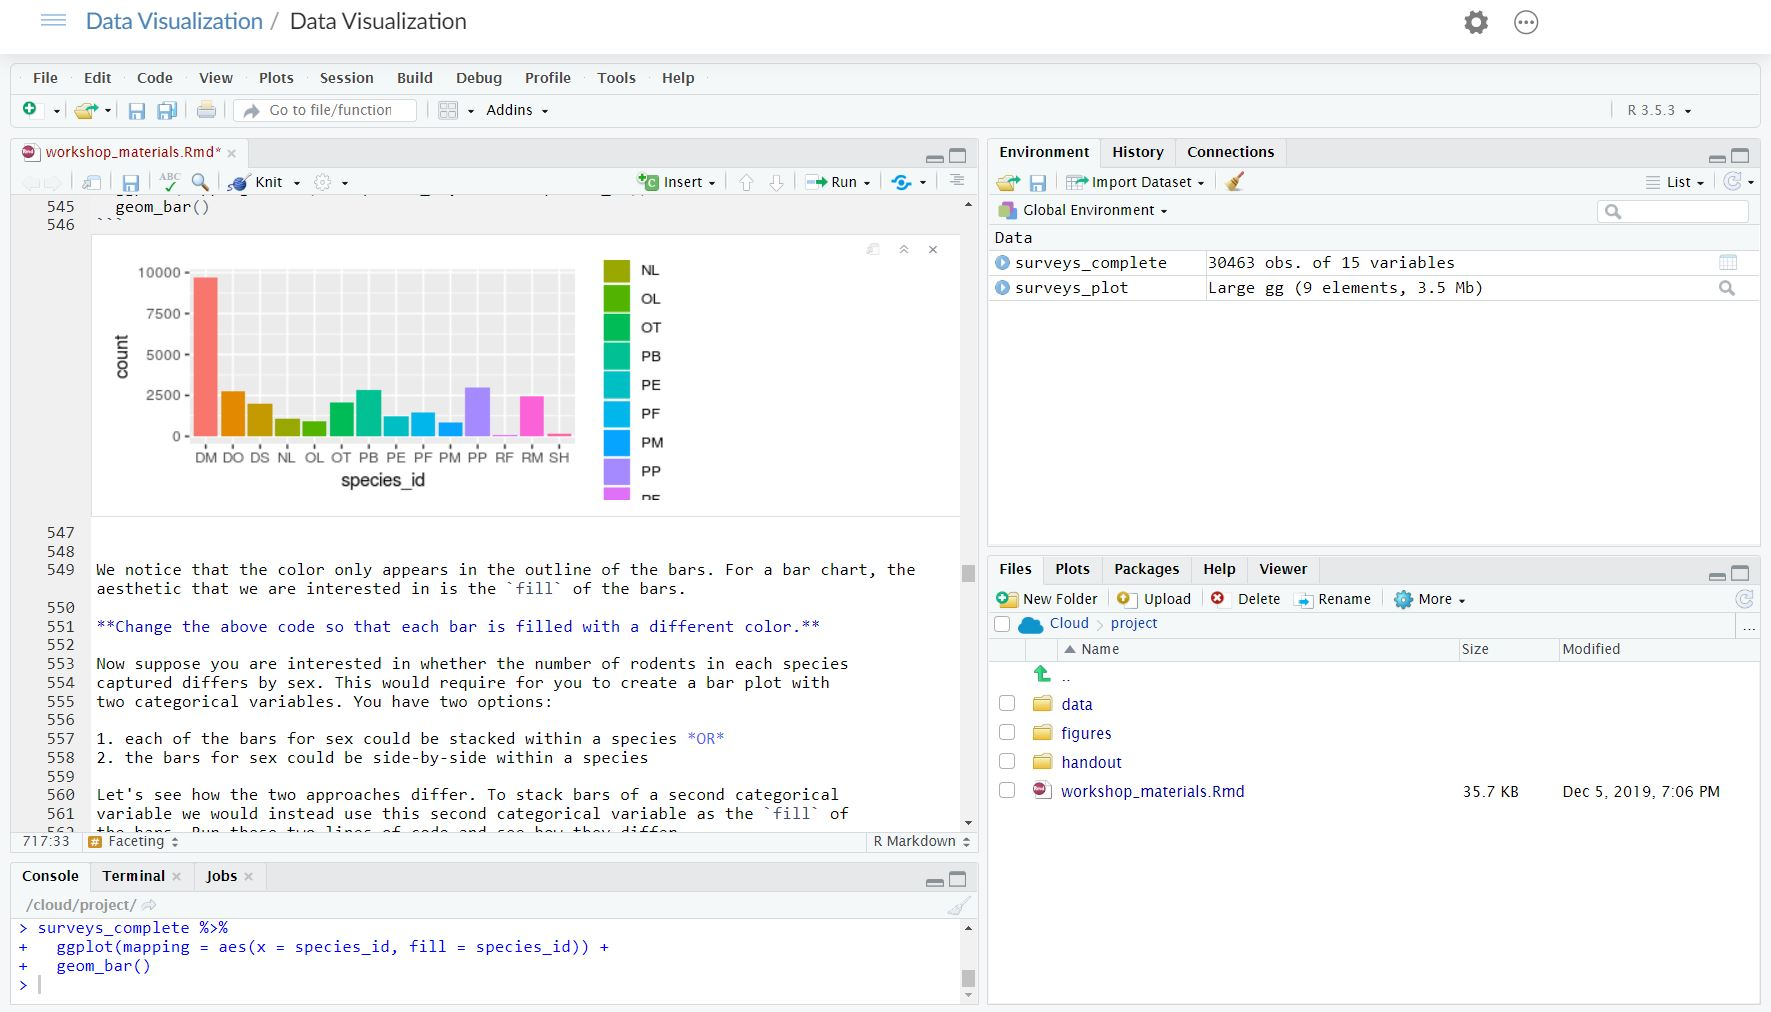
\includegraphics[width = \textwidth]{images/RStudio_Cloud_blind.png}
    \caption{RStudio Cloud workspace environment for \emph{Data Visualization with \texttt{ggplot2}} workshop. Every workshop works in an \texttt{R} project, containing a master \texttt{R Markdown} file, a data folder containing the data used in the workshop, and the handout produced for attendees.} 
    \label{fig:cloud}
\end{figure}

\subsubsection{Why R Markdown Documents?}

\quad The \texttt{rmarkdown} package \citep{rmarkdown} and its associated \texttt{R Markdown} documents provide an easy-to-understand framework for creating reproducible documents. \text{R Markdown} documents are able to combine statistical computing and written analyses into one reproducible document, helping to break the copy-paste paradigm for generating statistical reports. The workshop materials participants clone include a master \texttt{R Markdown} document containing blocks of code and descriptions for every topic covered throughout the workshop. Therefore, when participants revisit their materials, the code they generated is neatly organized alongside the description of the process the code carries out, decreasing the amount of ramp-up time when they revisit their materials at a later time. 

\quad During the workshop, \texttt{R Markdown} documents allow for attendees to keep their code organized and their workspace clean. For new learners, it is unnatural to create an organized script file with comments on each step. Furthermore, for these learners, it is difficult to understand the difference between generating \texttt{R} code in a script file versus executing code in the \texttt{R} console. An \texttt{R Markdown} file allows for participants' exploratory work to be saved within a topic's empty \texttt{R} code chunk, situating the code in context of each topic and helping workshop facilitators more easily debug any issues that may arise.   

\subsection{Workshop Content}

\subsubsection{Introduction to \texttt{R}}
\label{sec:introR}

\quad This first workshop in the series covers the basics of learning to program in \texttt{R}. The workshop first introduces the RStudio environment and project work flow in RStudio, discussing working directories and relative paths. Next, the workshop progresses through tools for working with vectors and lists of different data types, motivating methods for working with dataframes in \texttt{R}. After learning how to import data into \texttt{R}, the workshop proceeds through inspecting data, extracting data, and changing data types. Motivated by obtaining unexpected summary statistics when working with missing data, the workshop introduces \texttt{R} help files to inspect function arguments and their default values. These help files are called upon as participants use base \texttt{R} functions to create summaries of the data, perform basic data cleaning, and produce both univariate and bivariate visualizations of the data. 

\subsubsection{Intermediate \texttt{R}}
\label{sec:intermed}
% Add footnote link to GitHub repository 

\quad This second workshop in the series builds off of the content covered in \emph{Introduction to \texttt{R}}, without any expectations of attendees having additional knowledge or skills. The workshop begins with a review of creating objects in \texttt{R} and working with vectors and dataframes. The workshop then progresses through the use of relational statements in \texttt{R} and how to link these statements together using and (\texttt{\&}), or (\texttt{|}), and not (\texttt{!}) conjunctions. Next, the workshop dives into the use of conditional statements, stepping from \texttt{if}, to \texttt{if else}, to \texttt{else if} statements. 

\quad The second half of the workshop covers methods to iterate or replicate the same set of instructions many times. For-loops are introduced as a popular way to iterate or replicate the same set of instructions many times. Participants work through examples of a for-loop and a recursive for-loop, in the context of repeated operations on a dataset. These exercises motivate the discussion of why many \texttt{R} users recommend instead using vectorization for non-recursive for-loops. 

\quad Lastly, functions are presented as an approach to replicate the same set of instructions in multiple locations throughout your code. Persuaded by an \texttt{R} script which copies and pastes the same process multiple times, participants understand the difficulty in discerning the underlying process and spotting mistakes. Participants are then tasked with transforming this copy-paste process into a function. By parsing out the function writing process into a set of steps that one walks through once you've copied and pasted your code multiple times, participants have a more intuitive sense for why functions are useful and how they can create them in their own code.

\quad The content in this workshop, excluding relational statements, is not included in Data Carpentry's \emph{Data Analysis and Visualization in \texttt{R} for Ecologists} lesson. Instead, many of these concepts are covered in Software Carpentry's \emph{\texttt{R} for Reproducible Scientific Analysis} lesson. Yet, creating modularized code---which uses conditional statements, for-loops, and user-defined functions---are skills that many environmental science faculty asserted were necessary for graduate students to possess as they perform independent research.  


\subsubsection{Data Wrangling with \texttt{dplyr} and \texttt{tidyr}}
\label{sec:wrangle}

\quad Following the \emph{Intermediate \texttt{R}} workshop, the \emph{Data Wrangling} workshop continues forward with common data wrangling issues faced by environmental science researchers. Inspired by the difficulty of reading bracket subsetting and how cumbersome it can be to remember the different base \texttt{R} functions and formats to wrangle your data, this workshop introduces the \texttt{dplyr} \citep{dpylr} and \texttt{tidyr} \citep{tidyr} packages from the \texttt{tidyverse} \citep{tidyverse}. Much of \texttt{R}'s language has not changed over the last 20 years, which leaves the desire for a ``smoother, more efficient, and more readable pipeline for modern \texttt{R} workflows'' (Ross, Wickham, \& Robinson, \citeyear{tidytools}, p. 19). The \texttt{tidyverse} packages share common interfaces and data structures that make it simpler to learn data wrangling tasks and allow for the process to flow naturally from one step to the next. 

\quad The workshop begins with a description of the purpose of the \texttt{dplyr} package and an outline of six of the common ``verbs'' that handle common data wrangling challenges. Participants learn how to select columns with \texttt{select()}, filter rows with \texttt{filter()}, add new columns and modify existing columns with \texttt{mutate()}, create a table of summary measures by groups using \texttt{summarise()} and \texttt{group\_by()}, and change the ordering of a tables rows with \texttt{arrange()}. Prompted by the need to perform a sequence of multiple data wrangling operations, participants learn how to connect each of these data wrangling verbs using the pipe operator (\texttt{\%>\%}). 

\quad Next, the concept of relational data is outlined, impelled by the need to integrate additional data files for analysis. Participants are introduced to the idea of key-value pairs and then use these pairs to map how the data with which they have been working can be joined with additional data files. After discussing the four types of joins (inner, left, right, full), participants use the \texttt{left\_join()} and  \texttt{right\_join()} functions to join the three datasets used in the workshop. 

\quad The final topic of the workshop involves data reorganization, beginning with a discussion of ``tidy'' data. Up until now, the data were presented to participants in a ``tidy'' format, where every observation is one row, each variable has a column, and every value has one cell. This idea is then used to describe `long' and `wide' data formats, and a discussion around why each format may be useful ensues. The \texttt{tidyr} package is introduced to alleviate the burden of these types of data reorganizations, with an introduction to the \texttt{gather()} and \texttt{spread()} functions. In groups, participants then work through a final exercise applying the skills acquired throughout the entire workshop, starting with creating a data summary for multiple groups, then spreading the values across multiple columns, and finally recombining these multiple columns into a single column. 


\subsubsection{Data Visualization with \texttt{ggplot2}}
\label{sec:vizual} 

\quad The final workshop in the series dives into creating data visualizations using the \texttt{ggplot2} package \citep{ggplot}. Rather than remembering a list of functions that make different visualizations, each with it's own unique syntax, arguments, inputs, and outputs, \texttt{ggplot2} creates a uniform interface with functions that each solve a particular class of problems. This uniform syntax and set of functions allows participants to create more dynamic visualizations out of the gate. This workshop works with the joined data from the close of the \emph{Data Wrangling} workshop. We begin with participants executing code to generate a scatterplot, using \texttt{ggplot()}, which is then used to illuminate the discussion of the \texttt{ggplot()} syntax.

%\begin{verbatim}
%ggplot(data = <DATA>) +
%<GEOM_FUNCTION>(mapping = aes(<MAPPINGS>))
%\end{verbatim}

\quad Participants learn about the \texttt{mapping} argument for specifying aesthetics (\texttt{aes}) for the plot and the set of \texttt{geom} functions which define the type of plot you produce. By making explicit connections between the addition operator (\texttt{+}) and the pipe operator, participants understand addition to be an intuitive metaphor for adding layers to a plot. This discussion directly links to the concepts introduced in the previous workshop, using the pipe operator to motivate why the first argument of \texttt{ggplot()} is the data, and the `long' data format which \texttt{ggplot2} requires. 

\quad Next, the workshop examines how to modify the \texttt{ggplot()} aesthetics and geoms to create violin plots, density plots, bar charts, and line plots. Each of these plots allow for participants to explore different \texttt{geom} functions and the aesthetics that pair with each plot. A conversation is had about the importance of plotting raw data rather than simply aggregate measures of the data, by adding a \texttt{geom\_point()} or \texttt{geom\_jitter()} layer, further highlighting the layering possibilities in \texttt{ggplot()}. Finally, faceting is introduced as an additional tool for creating multivariate visualizations. Participants work with both the \texttt{facet\_wrap()} and \texttt{facet\_grid()} functions to create multiple subplots based on categorical variables from the data. 

\quad By this point in the workshop, participants have posed many questions on how to modify aspects of a plot that don't depend on the geom. For the final section of the workshop, the group walks through different customizations one can make to each \texttt{ggplot} object. Participants learn how to customize a plot's labels, the size of the points, the thickness of lines, the appearance of the plotting window, the color scheme used, and the size, color, and angle of the plot's labels. 

\quad Exporting graphics is the final topic of the workshop. At this point, attendees have generated numerous plots, including faceted and arranged plots, which could potentially be used as templates for graphical displays in their research. The workshop closes with a discussion of the difference between exporting a plot using the ``Export'' tab and using the \texttt{ggsave()} function. As participants may ultimately use the \texttt{ggplot} visualizations they create for publications, a discussion of plotting dimension and resolution is included. 


\subsection{Sustainability of Workshops}  

\quad To facilitate the sustainability of these workshops, we forged a partnership between our institution's library and the Department of Mathematical Science's Statistical Consulting and Research Services (SCRS). A university's library is an optimal unit for offering these workshops, as it is both department-agnostic and a central hub for the entire university community. Through a partnership with SCRS and a \$5,000 faculty excellence grant, a train-the-trainer model was developed and employed to train new graduate students in the fall of 2019 to lead the instruction of these workshops in the spring. Due to the widespread use of \texttt{R} across scientific fields, students from a variety of backgrounds hold the potential to be effective instructors,  encouraging participation in the workshops throughout their field. Additionally, these workshops require helpers to address issues participants may encounter during the workshop and to circulate during the ``hands-on'' exercises. Incorporating undergraduate students as workshop helpers provides them with teaching experiences, and allows for the possibility of students becoming lead or co-instructors as they progress through their program. 


\section{Evaluating Data Science Workshops}
\label{sec:implement}

\quad The final phase of this research explored the backgrounds and experiences of workshop attendees. For the first iteration of this research, attention was paid to understanding the backgrounds of the workshop attendees, their experiences learning \texttt{R}, their motivation for attending the workshop(s), and their experiences in each workshop. Evaluating the learning outcomes of these workshops is left as future research.  
\subsection{Data Collection}

\quad  In the week prior to the workshop, a survey is sent out to those registered for the workshop through a public Google Form. The pre-workshop survey details individuals' areas of study, current occupations, statistics and computer science experiences, participation in independent research, and their chosen method of storing any data they've collected. Following each workshop, attendees are asked to complete another survey. This post-workshop survey details the workshop participants' experiences in the workshop environment, their familiarity with the content covered in the workshop, their ability to implement the skills they learned, the best thing about the workshop, and what could use improvement. The content of these surveys was informed from the pre- and post-workshop surveys disseminated for Data and Software Carpentry workshops \footnote{This work is a derivative of the Carpentries pre- and post-workshop survey materials \href{https://github.com/carpentries/assessment/}{(https://github.com/carpentries/assessment/)}, used under CC BY \href{https://creativecommons.org/licenses/by/4.0/}{(https://creativecommons.org/licenses/by/4.0/)}.}, with revisions to the disciplines and occupations provided, and removal of questions regarding the degree of agreement with statements provided. The full pre- and post-workshop surveys are included as supplementary materials.

% \subsection{Data Analysis}
% 
% \quad At the close of each semester, attendees' answers to pre- and post-survey free response questions were qualitatively analyzed. For each of these questions, surveys were inspected and initial descriptive codes were created for each response. For the statistics experiences, descriptive codes were produced based on the the name of the course, the content of the course, and the reported course number and institution. Descriptive codes for what attendees attested they hoped to learn, what they enjoyed, and what they reported could be improved focused on the content and context of the response.   
% 
% \quad In the final production of analytical codes for each of these four questions, categories were created to be mutually exclusive, exclusive, and exhausting, where the name of the code authentically represented the attendees description \citep{merriam}. For example, one attendee stated they were hoping to ``improve my abilities to effectively use \texttt{R},'' which was assigned to the theme of ``interest in learning more about \texttt{R}.'' A participant reporting a ``very welcoming atmosphere and fun group of people'' was categorized as belonging to the theme of workshop atmosphere. Another attendee stated that ``more time was need to cover the workshop material adequately. And really, I personally do not mind a 4 hour session with a tea break in between,'' which was categorized to belong to the theme of time. 


\subsection{Backgrounds of Workshop Participants}

\quad The workshops tailored to environmental science graduate students, during phase two, were offered each semester of the 2018-2019 academic year. A workshop schedule was created prior to the start of each semester, with care taken to not overlap with any required graduate-level environmental science seminars. The schedule of workshops was then distributed to department administrative assistants in these environmental science disciplines, to be advertised to each department's students, faculty, and staff. Additionally, these workshops were advertised through the library and our institution's weekly news and events. 

\quad A total of 150 unique students, faculty, and staff attended at least one of the workshops. Many participants elected to return for the subsequent workshops, but nearly 70\% only attended the \emph{Introduction to \texttt{R}} workshop. A total of 65 individuals attended the \emph{Introduction to \texttt{R}} workshop, 40 attended \emph{Intermediate \texttt{R}}, and 20 attended each of the \emph{Data Wrangling} and \emph{Data Visualization} workshops.    

\quad The majority of the workshop attendees were in biological fields---from departments such as Land Resources and Environmental Sciences (LRES), Ecology, Plant Sciences, Animal and Range Sciences, Earth Sciences, and Biochemistry or Microbiology. The majority of workshop attendees were masters and doctoral students in these fields. It is worth noting that 12 faculty, staff, and postdocs also attended these workshops. Figure \ref{fig:departments} displays the department affiliations of the workshop attendees and their current occupation. 

{\spacingset{1.05}
\begin{figure}[h!]
\centering
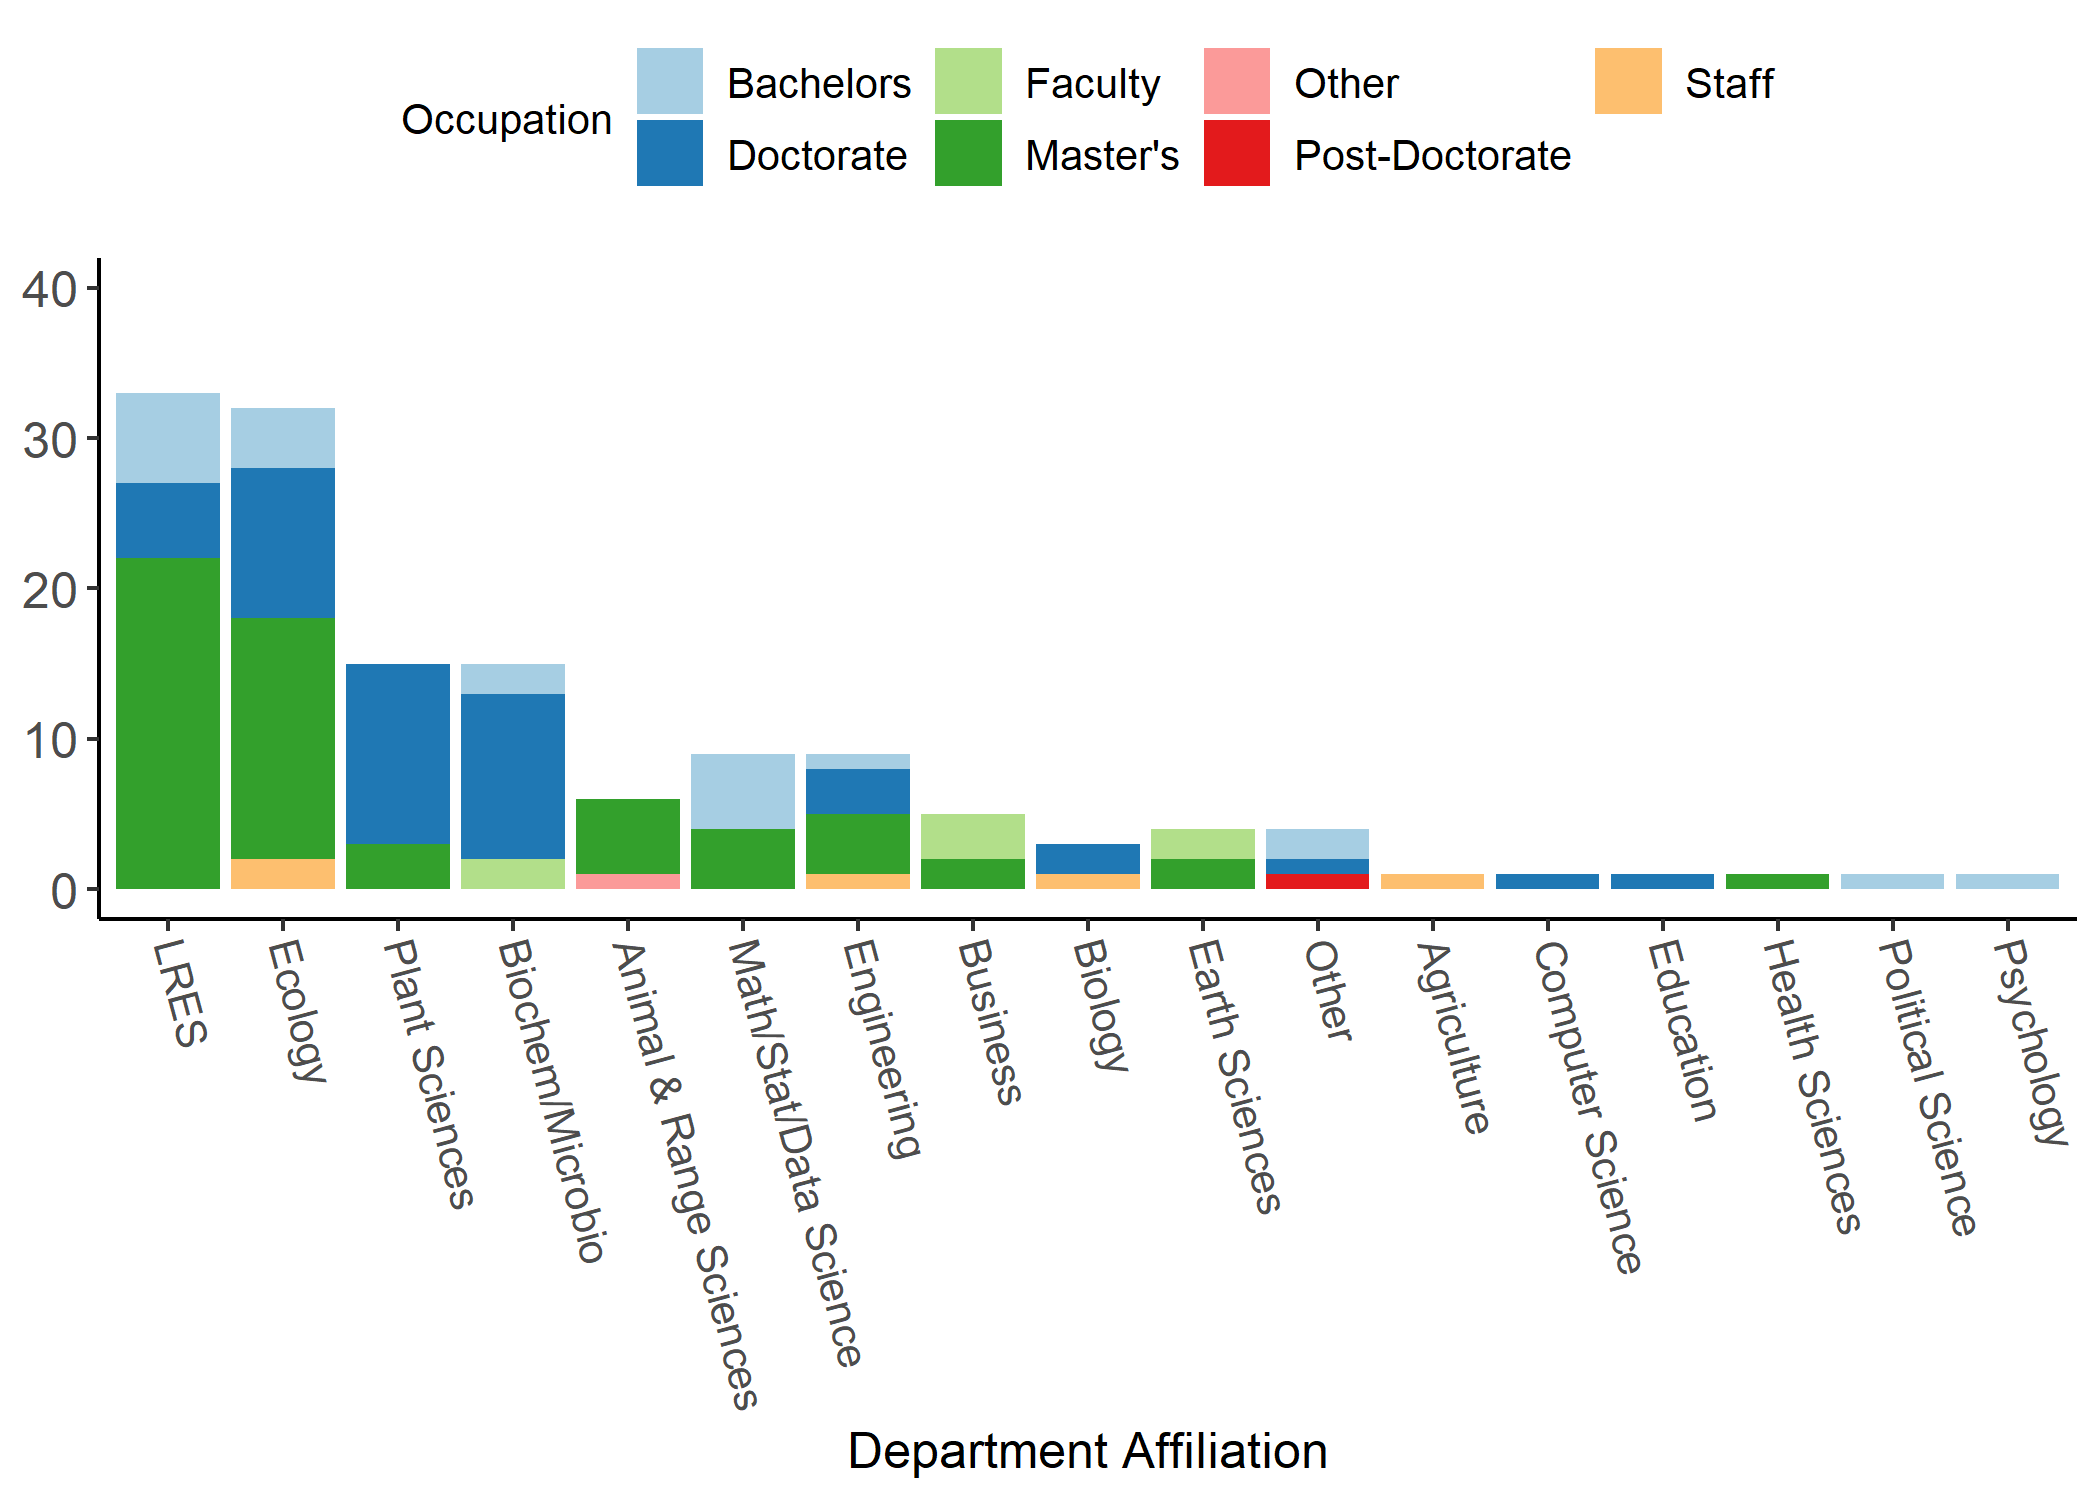
\includegraphics[width = \textwidth]{images/better_colors_attendance.png}
\caption{Number of attendees by department and current occupation, selected from an itemized list of campus departments and positions.}
    \label{fig:departments}
\end{figure}
}

\quad Consistent with the environmental science literature \citep{andelman, hampton, hernandez, datacarpentry}, a large number of workshop participants were either unfamiliar with the concept of a programming language or had no experience with any programming languages. As seen in Table \ref{tab:programming}, nearly 75\% of the attendees reported having never formally taken a course in computer programming.    \\

{\spacingset{1.05}
\begin{table}[h!]
    \centering
    \begin{tabular}{lc}
\hline
Programming Languages & Participants \\
\hline
What is a programming language? & 30 \\
None & 35 \\
\texttt{R} & 22 \\
SQL & 12 \\
Java or Javascript & 11 \\
C or C++ & 7 \\
Fortran & 4 \\
\hline
\end{tabular}
\caption{Workshop attendees' responses to the question of ``What programming languages do you have experience with? Select all that apply.''}
    \label{tab:programming}
\end{table}
}

\quad Many attendees, however, stated that they had taken courses in statistics. The majority of participants reported having some undergraduate of graduate experiences with introductory level statistics courses. Notably, over 15\% of attendees reported having no formal statistical training. Most graduate students had enrolled in discipline-specific introductory statistics courses in their own department or a graduate-level applied statistics course offered by the Department of Mathematical Sciences. Table \ref{tab:statistics} consolidates themes of workshop participants' previous statistical experiences, when asked to report the statistics courses they have taken over the course of their education. 

{\spacingset{1.05}
\begin{table}[h!]
    \centering
    \begin{tabular}{lc}
\hline
Stat Courses & Participants \\
\hline
Introductory Statistics & 46 \\
Applied Statistics & 42 \\
None & 24 \\
Discipline Specific Introductory Statistics & 20 \\
Intermediate Statistics & 10 \\
Experimental Design	& 8 \\
Probability Theory	& 6 \\
Statistical Computing & 3 \\
Sampling & 3 \\
Biostatistics & 2 \\
Spatial Analysis & 2 \\
Econometrics & 1 \\
Time Series Analysis & 1 \\
\hline
\end{tabular}
\caption{Workshop attendees' responses to the question ``What are your previous statistical experience(s)?  List course names.,'' thematically organized based on content of the course.}
    \label{tab:statistics}
\end{table}
}

\subsection{Motivation for Attending} 

\quad In Table \ref{tab:reasons} we outline what workshop participants reported as their ``most important reason for attending this workshop.'' As expected from the prevalence of the use of \texttt{R} in environmental science research \citep{Rpopular, mislan}, over half of the master's and doctoral workshop participants attended for assistance with their research. Others were seeking additional assistance for learning the \texttt{R} skills necessary for their coursework, refreshing or updating their \texttt{R} skills to include new tools they were unfamiliar with (e.g. \texttt{ggplot}, \texttt{dplyr}), or undergraduates preparing for graduate school.  

{\spacingset{1.05}
\begin{table}[h!]
    \centering
    \begin{tabular}{lc}
\hline
Reason Attended & Participants \\
\hline
Research assistance &  58 \\
Coursework assistance &  35 \\
Refresh or update skills &  16 \\
Department/Professor recommended &  13 \\
Preparation for graduate school &  12 \\
Professional Development &   7 \\
Adviser recommended &   6 \\
Expand Skills & 6 \\
\hline
\end{tabular}
\caption{Workshop attendees' responses to the question ``What is your most important reason for attending this workshop? Select all that apply.''}
    \label{tab:reasons}
\end{table}
}

\quad As echoed by previous studies of environmental science graduate students \citep{datacarpentry, theobold}, attendees overwhelmingly stated that they primarily use the internet, their peers, or their lab mates when learning \texttt{R}. Based on the statistical backgrounds of these participants and the statistics education literature on computing in the statistics classroom, it is not surprising that nearly two-thirds of these individuals reported using resources other than course materials as their main resource for learning \texttt{R}. Table \ref{tab:resources} details the resources workshop participants selected having used when learning to program in \texttt{R}. 

{\spacingset{1.05}
\begin{table}[h!]
    \centering
    \begin{tabular}{lc}
\hline
Resources Used to Learn \texttt{R} & Participants \\
\hline
Internet Resources & 55 \\
Peers & 43 \\
Course Materials & 35 \\
Lab Mates & 29  \\
Adviser	& 20 \\
These Workshops & 15 \\
Books & 3 \\
Professor & 1 \\
\hline
\end{tabular}
\caption{Workshop attendees' responses to the question ``What resources have you used while learning to program in \texttt{R}? Select all that apply.''}
    \label{tab:resources}
\end{table}
}

\quad The three themes which emerged from attendees' responses to ``what are you hoping to learn in this workshop?''  were requests specific to the content taught in the workshop, requests for content not applicable to the workshop. and general interest in learning about \texttt{R}. The number of participant responses to ` regarding the desire to learn more about \texttt{R} are indicative of the widespread use of \texttt{R} for data-intensive research. Furthermore, regardless of statistical background, the bulk of these workshop attendees voiced that they were hoping to learn \texttt{R} for some aspect of analyzing their data. On occasion these requests from attendees were out of focus of the broader workshop content, with requests to understand ``how \texttt{R} can be used to analyze microbiom data,'' ``geospatial analysis in \texttt{R},'' ``a refresher on stats,'' and ``how to integrate data into the \texttt{Ternary} package I'm learning.'' Given the backgrounds of workshop attendees, their reasons for attending, and the resources they've used to learn \texttt{R}, these workshop learning requests can be viewed as attendees cry for help. While other attendees' requests focused largely around the desire to learn \texttt{R} more fluently for their research---these specific requests for data analysis help could be attendees' final resort in understanding the analyses involved in their research.  

\subsection{Reflections of Workshop Participants} 

 \quad Every participant attending the workshops reported that they felt the workshop environment to be welcoming, with many participants voicing that the ``enthusiasm of the instructor'' was the best part of the workshop. The percentage of individuals reporting that all of the information presented was new to them differed by workshop, with 40\% of \emph{Introduction to \texttt{R}} participants, 30\% of \emph{Intermediate \texttt{R}} participants, 80\% in \emph{Data Wrangling}, and 50\% in \emph{Data Visualization}.
 
\quad The themes which emerged from these attendees' reflections to what they enjoyed most about the workshop were hands-on learning, workshop atmosphere, instructor attributes, and confidence. Many individuals commented on how walking through the code step-by-step made the information more clear, and how this process left them feeling more ``confident figuring things out on my own, now that I understand the general lay out and `way' commands or functions are set up.'' Furthermore, these participants voiced that the workshop left them with a more substantial feeling of independence, because ``I have a better understanding of how to read code, what certain symbols/terms/etc mean and how they work'' and ``I feel like I can better interpret [\texttt{ggplot}] code to work through it better individually now.'' Participants expressed that the hands-on exercises used throughout the workshops also contributed to ``fostering a much greater level of understanding.'' This deeper level of understanding was facilitated by providing participants with an adequate amount of time to ``explore \texttt{R} on our own'' and then spending time, as a group, talking through a variety of ways to address the task at hand. Some individuals who reported using the internet as a resource to learn \texttt{R} stated that ``it's easy to walk away from \texttt{R} workshops wondering if anything was learned, however the exercises were a clear tool which allow me to see what I gained.''  

\quad Across every workshop, nearly all participants stated that they ``strongly agreed'' that they ``learned skills that [they] will be able to use in [their] research/work.'' Over 75\% of the workshop participants reported that they would use the skills they learned in their research immediately or in the next 30 days. Numerous participants expressed that ``[in their field] the value of learning \texttt{R} cannot be underestimated,'' because ``[\texttt{R}] is an essential tool for researchers.'' While, a number of graduate students reflected on the importance of these workshops ``filling a critical hole in the curriculum of many college programs.'' Other students stated that they attended the workshops because they were taking a class which uses \texttt{R}, but had received no formal training in \texttt{R} at the start of the course. Therefore, as new \texttt{R} users, they felt that ``[they] were missing some of the most basic understanding,'' and the workshop left them ``feeling much more prepared to address the content in class now.''   

\quad Lastly, when attendees were asked what in the workshop needed to most improvement, themes of time and content appeared. The largest volume of constructive feedback from workshop participants focused on the amount of time allocated for the workshop. Many individuals stated that ``it could be better to have more time,'' suggesting an additional hour, with a ``break in between.'' However, others reflected that it could be more beneficial to have ``shorter, but more workshops,'' since ``it's easy for the brain to get tired after an hour or so.'' Due to the large attendance at many \emph{Introduction to \texttt{R}} workshops, often times a large number of questions would arise over the course of the afternoon. This lead to an inability to cover some of the workshop content in as much depth as hoped, which some participants remarked on. However, others felt that ``with so many people, [the workshop] had better discussions.'' There exists a balancing act between the amount of workshop content, the time allocated to addressing questions that may arise during the workshop, and the duration of the workshop. However, the three hours allocated to each of these workshops far exceeds the 60 minutes typically given to this content during a standard Data or Software Carpentry workshop. 

\section{Dissemination \& Future Directions} 

\quad Currently, this design research is focusing on incorporating the content of these workshops into the \emph{Data Analysis and Visualization in \texttt{R}} lesson within Data Carpentry's Ecology curriculum. Infusing the skills outlined in this research into the \emph{Data Analysis and Visualization in \texttt{R} for Ecologists} lesson helps to create a Carpentries curriculum that best reflects the ``core data skills'' necessary for data-intensive environmental science research. For skills outlined by this research where there is no room in the current \emph{Data Analysis and Visualization in \texttt{R} for Ecologists} lesson, the Carpentries Incubator and Carpentries Lab provide potential avenues to produce additional lesson materials that are broadly available to The Carpentries community. These avenues allow for the continued discussion of the importance of integrating user-defined functions, conditional statements, and loops into the broader Data Carpentry Ecology curriculum.    

\quad The next iteration of this design work will be informed by research concentrating on the computational skills employed by environmental science graduate students in their research code. Collecting the research (\texttt{R}) code produced by graduate students in the environmental sciences provides insight into the key computational skills students are using to implement statistics in their research. The skills outlined by this research aid in re-evaluating the content of these workshops, to ensure they cover the skills necessary for graduate-level environmental science research. 

\quad The attendance of these workshops by students, faculty, and staff from disciplines outside of the environmental sciences brings to question whether this type of tailored design work is necessary. While these workshops were originally designed to facilitate environmental science graduate students' acquisition of computing skills, over a third of the workshop attendees came from disciplines outside of this focus. Strikingly, these attendees reported similar workshop experiences to attendees from these targeted disciplines. This brings to question if there are common computational understandings necessary for research in \emph{any} scientific field, which should be infused into \emph{every} statistics and data science course. 

\quad Alternatively, in this research we saw a larger number of attendees from environmental science fields persist across workshops, rather than solely attending \emph{Introduction to \texttt{R}}. What are the drivers behind these individuals' continued attendance? Future research focusing on the learning outcomes of the workshop attendees could provide fruitful insight on the necessity of these discipline-specific learning opportunities. 

\section{Conclusion}
\label{sec:conclusion}

\quad Ten years ago, Nolan and Temple Lang declared that ``modernizing the statistics curricula to include computing [...] is an issue that deserves widespread attention and action'' (p. 106). In 2014, the American Statistical Association endorsed a new set of curriculum guidelines for undergraduate programs in statistical science. These new guidelines include an increased emphasis on data science skills and real applications, specifically students' ability to ``access and manipulate data in various ways, use a variety of computational approaches to extract meaning from data, program in higher-level languages" \citep[p. 7]{asa}. While we may see these changes reflected in undergraduate and graduate programs in statistics, integrating these topics into graduate-level statistics service courses has received less attention and poses different issues. 

\quad Statistics courses that serve a variety of students (undergraduate, graduate, statistics major, non-major) reflect a snapshot of the statistics curriculum, but often act as many students' sole statistics course prior to conducting scientific research. Instructors of these courses thus grapple with difficult decisions of how they can ensure their students have both the statistical and ``computational understanding, skills, and confidence needed to actively and wholeheartedly participate'' in the scientific research arena \citep[p. 106]{nolan}. For instructors unfamiliar with students' scientific disciplines, it can be difficult to ``be bold and design curricula from scratch'' \citep[p. 106]{nolan}.  

\quad The topics suggested by Nolan and Temple Lang (2010), represent a starting point towards building a taxonomy for computing in statistics for undergraduate and graduate statistics programs. These topics, however, may not be relevant to or emphasized by other scientific disciplines whose students enroll in graduate-level statistics service courses.  In our research, we found that environmental science faculty stressed the importance of graduate students developing skills surrounding the fundamentals of working with data in \texttt{R}, software skills for data processing and preparation, creation of data visualizations, and usage of reproducible work flows. This research equips statistics service course instructors with knowledge of the computing skills necessary for data-intensive environmental science research, and facilitates a meaningful integration of computing topics into these types of courses.   

\quad Workshop participants' attribution of the internet, their peers, and lab mates as the resources they've used to learn \texttt{R} suggests that statistics courses continue to under prepare students with the computing understandings and skills necessary to ``engage in and succeed at statistical inquiry'' \citep[p. 97]{nolan}. Furthermore, the content covered by these workshops has been voiced by workshop participants to be extremely important and impactful, stating that the content covered in these workshops ``fills a critical hole in the curriculum of many college programs.'' 

\quad As we work toward a more thorough integration of computing into the statistics curriculum, this research offers a model for facilitating external workshops---promoting university-wide data science literacy. External workshops create opportunities every semester for a university's students, faculty, and staff to acquire computational skills in a hands-on, interactive environment. Moreover, these workshops provide avenues for faculty to acquire computing knowledge and skills ``they have not had the opportunity to learn well" \citep[p. 106]{nolan}, and provide resources and tools for instructors to integrate computing into their classroom.

\section{Acknowledgements}

We would like to specially thank the participants from this study, without whom this research would not have been possible. We would also like to thank the workshop helpers for their time and assistance, helping to grow the data literacy across our campus. 


\bibliography{ref}
\bibliographystyle{apalike}

\end{document}
